\documentclass[twoside,10pt]{article}

\usepackage[labelsep=period,textfont=it]{caption}
\captionsetup[table]{name=TABLE}
\renewcommand{\thetable}{\Roman{table}}
\usepackage{lipsum,booktabs}
\usepackage[super]{natbib}
\usepackage{lipsum} % Package to generate dummy text throughout this template
\usepackage[sc]{mathpazo} % Use the Palatino font
\usepackage[T1]{fontenc} % Use 8-bit encoding that has 256 glyphs
\linespread{1.00} % Line spacing - Palatino needs more space between lines
\usepackage{microtype} % Slightly tweak font spacing for aesthetics
\usepackage{derivative}
\usepackage[hmarginratio=1:1,top=32mm,columnsep=20pt]{geometry} % Document margins
\usepackage{multicol} % Used for the two-column layout of the document
%\usepackage[hang, small,labelfont=bf,up,textfont=it,up]{caption} % Custom captions under/above floats in tables or figures
\usepackage{booktabs} % Horizontal rules in tables
\usepackage{float} % Required for tables and figures in the multi-column environment - they need to be placed in specific locations with the [H] (e.g. \begin{table}[H])
\usepackage{hyperref} % For hyperlinks in the PDF
\usepackage{multirow}
\usepackage{graphicx}
\usepackage{amsmath}
\usepackage{amsfonts}
\usepackage{amssymb}
\usepackage{lettrine} % The lettrine is the first enlarged letter at the beginning of the text
\usepackage{paralist} % Used for the compactitem environment which makes bullet points with less space between them
\usepackage{xcolor}
\usepackage{abstract} % Allows abstract customization
\renewcommand{\abstractnamefont}{\normalfont\bfseries} % Set the "Abstract" text to bold
\renewcommand{\abstracttextfont}{\normalfont\small\itshape} % Set the abstract itself to small italic text

\usepackage{titlesec} % Allows customization of titles
\renewcommand\thesection{\Roman{section}} % Roman numerals for the sections
\renewcommand\thesubsection{\Roman{subsection}} % Roman numerals for subsections
\titleformat{\section}[block]{\large\scshape\centering}{\thesection.}{1em}{} % Change the look of the section titles
\titleformat{\subsection}[block]{\large}{\thesubsection.}{1em}{} % Change the look of the section titles

\usepackage{fancyhdr} % Headers and footers
\pagestyle{fancy} % All pages have headers and footers
\fancyhead{} % Blank out the default header
\fancyfoot{} % Blank out the default footer
\fancyhead[C]{Electron Spin Resonance $\bullet$ December 12, 2021 } % Custom header text
\fancyfoot[RO,LE]{\thepage} % Custom footer text


%----------------------------------------------------------------------------------------
%	TITLE SECTION
%----------------------------------------------------------------------------------------

\title{\vspace{-15mm}\fontsize{15pt}{10pt}\selectfont\textbf{Electron Spin Resonance}} % Article title

\author{
	\small
	\textsc{Lauren Hernandez, Kathryn Wong}\\[1mm] % Your name
	\normalsize \textit{University of Houston}\\ % Your institution
	\normalsize \textit{Physics 3313: Advanced Laboratory I}\\ % Your Course
	%	\normalsize \href{mailto:john@smith.com}{john@smith.com} % Your email address
	\vspace{-10mm}
}
\date{}

%----------------------------------------------------------------------------------------

\begin{document}
	
	\maketitle % Insert title
	
	\thispagestyle{fancy} % All pages have headers and footers
	
	%----------------------------------------------------------------------------------------
	%	ABSTRACT
	%----------------------------------------------------------------------------------------
	
	\begin{abstract}
		
		\noindent The goal of this experiment is to use electron spin resonance to measure the spin magnetic moment of an electron. The spin magnetic moment was calculated to be $1.0636 \cdot 10^{-29}$. The signal height versus angle between the axis of the probe and the direction of the external magnetic field is proportional to $\sin^2\theta$. The small fixed magnet caused a change in the absorption peaks, because the magnet changed the magnetic field, which proportionally changed the voltage generated by the system.
		
		
	\end{abstract}
	
	%----------------------------------------------------------------------------------------
	%	INTRODUCTION
	%----------------------------------------------------------------------------------------
	
	\begin{multicols}{2} % Two-column layout throughout the main article text
		
		\section{Introduction} 
		
		\lettrine[nindent=0em,lines=2]{T}he term electron spin resonance comes from an atomic situation where there are a greater amount of electrons at a lower energy level within an atom. The population of low energy level electrons exhibit a net absorbption of energy rather than emitting energy. The transitions of electrons in a spin state are then in resonance with the difference in the interaction potential energy, which is source of the term ESR. Applications of ESR are significant in analyzing paramagnetic structures, the electronic structure of free radicals, and gathering kinetic and thermodynamic data. 
		
		\indent The goal of this experiment is to use electron spin resonance to measure the spin magnetic moment of an electron. An external magnetic field is applied to an atom in order to split the atomic energy level, specifically the ground state energy level, in two. The external magnetic field is provided by two Helmholtz coils and can be calculated using the following equation:
		
		\begin{equation}
		\vec{B_0} =\bigg( \frac{4}{5}\bigg)^{3/2}(\vec{\mu_0} N \vec{I})/a, 
		\end{equation}
		
		 \noindent where $\vec{B_0}$ is the magnetic field, $\vec{\mu_0}$ is the permeability of free space, $N$ is the number of turns in the coil, and $\vec{I}$ is the current in each coil. However, since the two coils are set up in parallel, $N = 60$ and $a = 0.056m$, then the magnetic field at the center of the coils is:
			
		\begin{equation}
		\vec{B} =0.48 \vec{I} (m T),
		\end{equation}
		
		
		\noindent where $\vec{I}$ is the current running through the coils. The atom is exposed to a second magnetic field caused by low amplitude radio frequency waves, and either the applied magnetic field or the frequency of the radio waves are adjusted until resonance occurs. Resonance is indicated whenever $\vec{B_0}$ is such that:
		
		\begin{equation}
			h \nu_R = 2 \vec{\mu_s} \vec{B_0},
		\end{equation}
		
		\noindent where $h = 6.626 \text{x} 10^{-34} \text{J} \cdot \text{s}$, $\nu_R$ is the resonant frequency, 
		$\vec{\mu_s}$ is the spin magnetic moment, and $\vec{B_0}$ is the applied magnetic field. Further, the spin magnetic moment can be calculated due to the following relationship:
		
		\begin{equation}
		\triangle U = 2 \mu_s B_0 = h\nu_R,
		\end{equation}
		
		where $\triangle U$ is the difference in interaction potential energy, $\mu_s$ is the spin magnetic moment, $B_0$ is the applied magnetic field, $h = 6.626 \text{x} 10^{-34} \text{J} \cdot \text{s}$, and $\nu_R$ is the resonant frequency. Once $\triangle U$ and $\vec{B_0}$ are known, the spin magnetic moment of the electron can be determined. 
		
		
		%	EXPERIMENTAL PROCEDURE
		%----------------------------------------------------------------------------------------
		
		\section{Experimental Procedure}
		
		\subsection*{Equipment}
		We used two small magnets, a standard plastic compass, two WT banana wires, a five pin DIN Cable BELDEN 148444, two BNC Cables KEITHLEY Instruments 4801 and BELDEN 28250, a Tripp Lite extension cord, two alligator clips, an Agilent 54621A Oscilloscope, two standard cable wires, a Daedalon Corporation ESR Power Supply, an EXTECH EX430A multimeter, an ESR Head EN-35/p Probe 0050, and two Conco Helmholtz Coils. 

		\subsection*{Procedure}
		
		\indent We connected the Helmholtz coils to the banana jacks on the back of the base unit. The ESR Head was already connected to the ring stand, so we left that as is. We connected the head to the base unit using the five pin DIN cable, and connected the BNC cable to the frequency jack on the base unit. We connected the other BNC cable from the ESR head to the Y input on the oscilloscope, and we connected the Helmholtz coil's sense jack to the oscilloscope's X channel input. We put the probe into the ESR head and put it through the Helmholtz Coils. We turned on the base unit, the head, and the oscilloscope, setting it to X-Y mode. We set the X-scale to 2V/cm and we set the Y-scale to be between 50mV/cm and 1V/cm; we also set both X and Y inputs to DC. 
		
		\indent Once the system was connected and on, we turned the Coil Current Adjust control to max, resulting in two visible peaks on the display. We increased the amplitude of the peaks by turning down the feedback control knob. Then, we turned the Feedback Control knob fully clockwise, and then turned the Tuning Control knob clockwise until the display was almost to zero. We adjusted the Tuning Control knob counterclockwise, until we determined the lowest frequency the oscillator could make. We kept the oscillator at this lowest frequency, and then measured the distance between the two amplitude peaks. We repeated this measurement ten times for ten more oscillator frequencies. Then, we selected a midrange frequency and adjusted the Feedback Control knob until we got the largest peaks possible. We collected data for signal height and $\theta$, where $\theta$ is the angle between the Helmholtz Coils and the Oscillator Head, ranging from $0^{\circ} - 90^{\circ}$. Lastly, we observed the effects on the position and signal height of the peaks when small magnets were introduced to the system. We introduced the magnets to the system from every possible direction, and for each polarity of the magnet. 

		
		%----------------------------------------------------------------------------------------
		%	RESULTS, ANALYSIS AND DISCUSSION
		%----------------------------------------------------------------------------------------
		\section{Results, Analysis, Discussion}
		
		The largest value of $\nu_r$ that the oscillator produced was 31.86 mHz, and the potential difference (2V), $2B_{0-Res}$, was 3.8 V. Shown below in Table 1 is the data collected for the potential difference between absorption peaks with a varying frequency. 
		
			\begin{table}[H]
			\centering
			\caption{The potential difference between two absorption peaks, measured as 2V, recorded for an increasing frequency over a uniform step size of approximately 0.886mHz.  }
			\begin{tabular}{l c c rrrrrrr}
				\toprule				
				Frequency (mHz) & 2V ($2 B_{0 - Res}$)  \\ [1ex]
				\midrule
			$23.00 \pm 0.01	$ &	3.8  V  \\ [1.5ex]
			$ 23.85 \pm 0.01$	&	3.9 V \\ [1.5ex]
			$ 24.70 \pm 0.01$	&	4.0 V  \\ [1.5ex]
			$25.62 \pm 0.01$  & 4.1 V \\ [1.5ex]
			$26.52 \pm 0.01$  & 4.2V \\ [1.5ex]
			$27.42 \pm 0.01$ & 4.2 V \\ [1.5ex]
			$ 28.30 \pm 0.01 $ & 4.3 V \\ [1.5ex]
			$ 29.18 \pm 0.01$ & 4.4 V \\ [1.5ex]
			$ 30.08 \pm 0.01$ & 4.5 V  \\ [1.5ex]
			$30.96 \pm 0.01$ &  4.6 V \\ [1.5ex]
			$31.85 \pm 0.01$ & 4.7 V \\ [1.5ex]
			
				\bottomrule
			\end{tabular}
		\end{table}
	
	Figure 1 shows the relationship between oscillator frequency and the resonant magnetic field. 
	
		\begin{figure}[H]
		\centering
		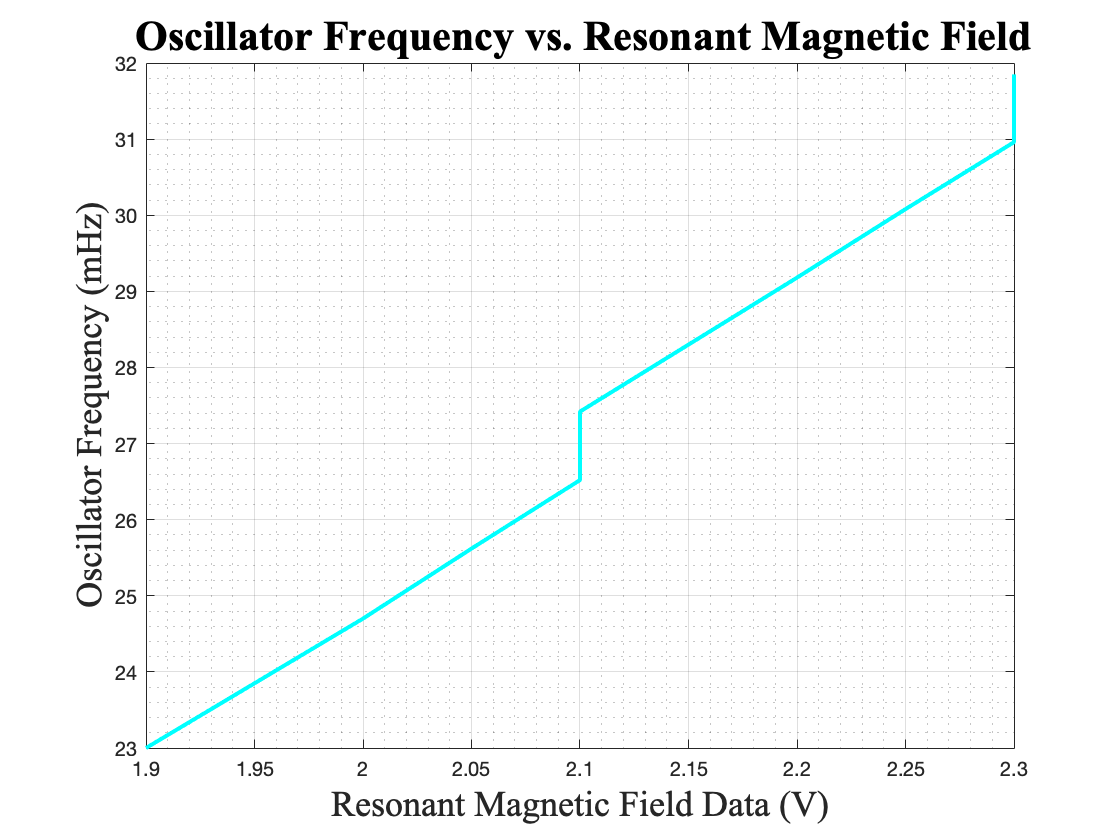
\includegraphics[width=\linewidth]{oscillator_vs_field.png}
		\caption{The relationship between the oscillator frequency and the resonant magnetic field between the two absorption peaks.  }
	\end{figure}

     Figure 1, as shown above, displays the relationship between the oscillator frequency and the resonant magnetic field. By using the relationship in equation 4, the spin magnetic moment was calculated to be $1.0636 \text{x} 10^{-29}$. This part of the experiement could have been negatively effected by errors due to parallax while reading the oscilloscope display. 

			\begin{table}[H]
	\centering
	\caption{ Signal height of the two absorpton peaks when the angle between the two Helmholtz Coils and the Oscillator head varies between $0^{\circ} - 90^{\circ}$.}
	\begin{tabular}{l c c rrrrrrr}
		\toprule				
		$\theta$ (degrees) & Signal Height (mV)  \\ [1ex]
		\midrule
		0 &	43.8  \\ [1.5ex]
		9	&	40.6 \\ [1.5ex]
		18	&	39.1  \\ [1.5ex]
		27  & 34.4 \\ [1.5ex]
		36  & 32.8 \\ [1.5ex]
		45 & 29.7 \\ [1.5ex]
		54 & 23.4 \\ [1.5ex]
		63 & 20.3 \\ [1.5ex]
		72 & 17.2  \\ [1.5ex]
		81 &  15.6 \\ [1.5ex]
		90 & 9.4 \\ [1.5ex]
		
		\bottomrule
	\end{tabular}
\end{table}


		\begin{figure}[H]
	\centering
	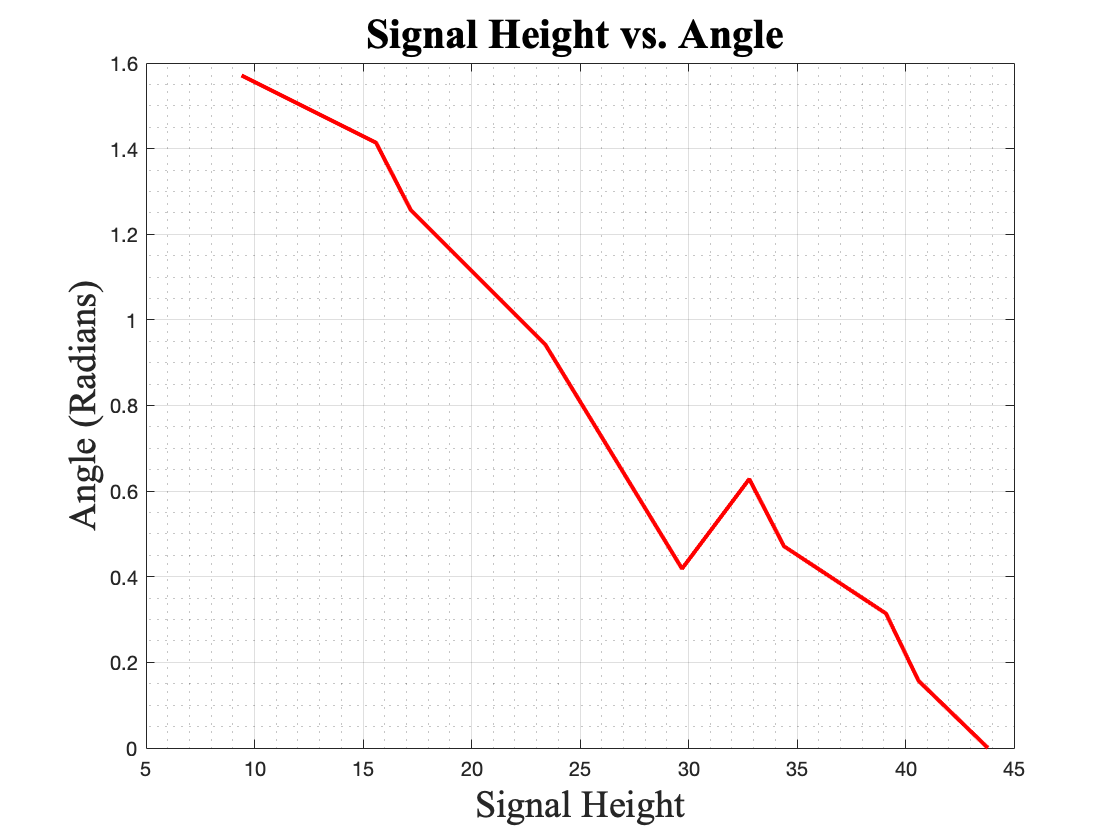
\includegraphics[width=\linewidth]{angle_vs_height.png}
	\caption{ The relationship between signal height and the angle between the axis of the oscillator coil and the direction of the external magnetic field. }
\end{figure}


The data collected confirms that the signal height is proportional to $\sin^2\theta$, where $\theta$ is the angle between the probe and the direction of the external magnetic field. We can confirm this proportionality by observing Figure 2, shown above, where the slope of the curve corresponds to the relationship between the angle and the signal height; the signal height decreases proportionally to the angle. We could have improved on the exactness of this part of the experiment if we had of gathered more data points for the curve. 

\indent When we introduced the small magnets to the Helmholtz Coil system, we observed that the south pole ,x-axis of the magnet increases the amplitude of the signal, and shifts the peaks to the left; we observed that the north pole, x-axis of the magnet decreases the amplitude of the signal, and shifts the peaks to the right. We observed that the north pole, y-axis of the magnet increases the amplitude of the two peaks, and shifts the peaks inwards towards each other; the south pole, y-axis of the magnet has the same effect as the aforementioned magnet angle, direction combination. We observed that the north pole, z-axis of the magnet increases the amplitude of the two peaks, ans as the magnet gets closer to the coils, the peaks combine and collapse at zero; the same behavior was observed for the south pole, z-axis. The introduction of the magnet to the external oscillating field causes a deflection in the absorption peaks, because the magnet changes the direction of the magnetic field of the Helmholtz coils; the magnetic field of the Helmholtz coils is no longer uniform. This is related to Faraday's law, where the voltage generated is linearly dependent on the external magnetic field. The effect on the Lande factor would be different if the small magnet was replaced with a crystalline sample. A magnet will have a greater tendency to align with a magnetic field due to it's composition, whereas a crystalline sample with a magnetic field will not be as strong due to the interaction between the neighboring atoms inside the crystal$^1$.. It's helpful to understand that the magnetism of a substance is composed of the magnetic moments of its atoms$^2$. This part of the experiment could have been more interesting if we had a very large magnet to introduce to the Helmholtz coil system. This would have allowed us to observe deflections in the absorption peaks to a greater, more dramatic magnitute. 
		
		
		%----------------------------------------------------------------------------------------
		%	CONCLUSIONS
		%----------------------------------------------------------------------------------------
		\section{Conclusion}
		The goal of this experiment was to use electron spin resonance to measure the spin magnetic moment of an electron; the spin magnetic moment was calculated to be $1.0636 \cdot 10^{-29}$. The signal height versus angle between the axis of the probe and the direction of the external magentic field is confirmed to be proportional to $\sin^2\theta$. The small fixed magnet caused a change in the absorption peaks, because the magnet changed the magnetic field, which proportionally changed the voltage generated by the system, according to Faraday's Law. 
		
		
		
		%	REFERENCE LIST
		%----------------------------------------------------------------------------------------
		\begin{thebibliography}{99} % Bibliography - this is intentionally simple in this template
			\raggedright
			\bibliography{mybib}
			\begin{small}
				\bibitem[1]{2001}
			Encyclopædia Britannica, inc. (n.d.). Magnetism. Encyclopædia Britannica. Retrieved December 12, 2021, from https://www.britannica.com/science/crystal
			/Magnetism. 

				
				\bibitem[2]{2002}
				What's magnetic moment? Stanford Magnets. (2020, October 14). Retrieved December 12, 2021, from https://www.stanfordmagnets.com/whats-magnetic-moment.html. 

			\bibitem[3]{2003}
			Ulinski, A. \& Forrest, R. L., "Lab Manual for Advanced Laboratory I", Physics 3313, \textit{Electron Spin Resonance}, pages 1 - 6, (The University of Houston, 2021).
			\end{small}
			
			
		\end{thebibliography}
		
		%----------------------------------------------------------------------------------------
		
	\end{multicols}
	
\end{document}